\documentclass[letterpaper, 12pt]{article}

%%%%%%%%%%%%%%%%%%%%%%%%%%%%%
% DEFINITIONS
\gdef\mytitle{M\"undliche Matura}
\gdef\mythema{Datamining \& Datawarehousing}

\gdef\mysubject{INSY}
\gdef\mycourse{5AHITM 2015/16}
\gdef\myauthor{Daniel Melichar}
\gdef\myversion{0.1}
\gdef\myteacher{Betreuer: Michael Borko}

%%%%%%%%%%%%%%%%%%%%%%%%%%%%%%
% SETTINGS
%!TEX root=../document.tex

\usepackage[in]{fullpage}
% Fontencoding for possible copy&paste out of PDF
\usepackage[T1]{fontenc}
\usepackage[utf8x]{inputenc}
\usepackage[english]{babel}
\usepackage{graphicx} 
\usepackage{textcomp}
\usepackage{sectsty}
\usepackage{caption}
\usepackage{listings}
\usepackage{array}
\usepackage{colortbl}
\usepackage{footmisc}
\usepackage{fancyhdr}
\usepackage{ccicons}
\usepackage{suffix}
\usepackage{multirow}
\usepackage{tabularx}
\usepackage{listings}
\usepackage{color}
\usepackage{url}
\usepackage[toc]{glossaries}
\usepackage[dvipsnames]{xcolor}
\usepackage[longnamesfirst,nonamebreak]{natbib}
\usepackage[headsep=1cm,headheight=3cm,hmargin=2cm,vmargin=2.5cm]{geometry}
\usepackage[nolist]{acronym}

% Definitions for Textcolor
\usepackage{color}
\definecolor{listings}{rgb}{0.96, 0.96, 0.96}
\definecolor{update}{rgb}{1, 0.8, 0.8}
\definecolor{config}{rgb}{0.8, 1, 0.8}
\definecolor{gray}{rgb}{0.4,0.4,0.4}
\definecolor{darkblue}{rgb}{0.0,0.0,0.6}
\definecolor{cyan}{rgb}{0.0,0.6,0.6}

% Java Syntaxhighligthning
% strings
\definecolor{javared}{rgb}{0.6,0,0}
% comments
\definecolor{javagreen}{rgb}{0.25,0.5,0.35}
% keywords
\definecolor{javapurple}{rgb}{0.5,0,0.35}
% javadoc
\definecolor{javadocblue}{rgb}{0.25,0.35,0.75}

\lstset{
	basicstyle=\ttfamily\small,
	keywordstyle=\bfseries\color[rgb]{0.496,0.000,0.332},
	commentstyle=\color[rgb]{0.246,0.496,0.371},
	stringstyle=\color[rgb]{0.164,0.000,0.996},
	tabsize=4,
	breaklines=true,
	numbers=left,
	numberstyle=\tiny\color{black},
	stepnumber=5,
	numbersep=10pt,
	numberstyle=\tiny,
	captionpos=b,
	xleftmargin=1cm,
	showspaces=false,
	showstringspaces=false,
	basewidth={0.53em,0.45em},
	frame=single,
	xleftmargin=1cm,
	basicstyle=\scriptsize,
}


\lstdefinestyle{Java}{
	language=Java,
	keywordstyle=\color{javapurple}\bfseries,
	stringstyle=\color{javared},
	commentstyle=\color{javagreen},
	morecomment=[s][\color{javadocblue}]{/**}{*/},
}

\lstdefinestyle{XML}{
	language=XML,
	basicstyle=\ttfamily,
	columns=fullflexible,
	commentstyle=\color{gray}\upshape
}

\lstdefinelanguage{XML}
{
	morestring=[b]",
	morestring=[s]{>}{<},
	morecomment=[s]{<?}{?>},
	stringstyle=\color{black},
	identifierstyle=\color{darkblue},
	keywordstyle=\color{cyan},
	% list your attributes here
	morekeywords={xmlns,version,type}
}

\usepackage[
	colorlinks,
	citecolor=black,
	filecolor=black,
	linkcolor=black,
	urlcolor=black,
	linktoc=all
]{hyperref}


% Useful Commands
% Comments and notes
\newcommand{\comment}[1]{}
\newcommand{\ifreport}[1]{#1}
\newcommand{\todo}{{\bf \colorbox{red}{\color{white}TODO:}}}
\newcommand{\ie}{{\em i.e.,~}}
\newcommand{\eg}{{\em e.g.,~}}
\newcommand{\term}[1]{\mbox{\texttt{#1}}}
\newcommand{\itl}[1]{\mbox{\textit{#1}}}

% Commas and semicolons
\newcommand{\comma}{,\,}
\newcommand{\commadots}{\comma \ldots \comma}
\newcommand{\semi}{;\mbox{;};}
\newcommand{\semidots}{\semi \ldots \semi}

% Brackets
\newcommand{\set}[1]{\{#1\}}
\newcommand{\sbs}[1]{\lquote #1 \rquote}

% Spacing
\newcommand{\gap}{\quad\quad}
\newcommand{\biggap}{\quad\quad\quad}
\newcommand{\nextline}{\\ \\}
\newcommand{\htabwidth}{0.5cm}
\newcommand{\tabwidth}{1cm}
\newcommand{\htab}{\hspace{\htabwidth}}
\newcommand{\tab}{\hspace{\tabwidth}}
\newcommand{\linesep}{\ \hrulefill \ \smallskip}

\setcounter{secnumdepth}{5}

\lhead{\mysubject}
\chead{}
\rhead{\bfseries\mythema}
\lfoot{\mycourse}
\cfoot{\thepage}
% Creative Commons license BY
% http://creativecommons.org/licenses/?lang=de
\rfoot{\ccby\hspace{2mm}\myauthor}
\renewcommand{\headrulewidth}{0.4pt}
\renewcommand{\footrulewidth}{0.4pt}

%%%%%%%%%%%%%%%%%%%%%%%%%%%%%
% DOCUMENT BEGIN
\begin{document}
\parindent 0pt
\parskip 6pt

% TITLE PAGE
%!TEX root=../laborprotokoll.tex

\begin{titlepage}

	\begin{figure}[!h]
		\begin{flushright}
			
\includegraphics[width=0.3\linewidth]{images/jdIT_tgm.png}
		\end{flushright}
	\end{figure}

	\vspace{2.5cm} 

	{\begin{center} \bfseries\huge
			\rule{17.5cm}{0.1mm}  
			\\[5mm]
			\mytitle\\[5mm]
			\mythema\\
			\rule{17.5cm}{0.1mm}  
	\end{center}}

	{\begin{flushright} \bfseries\Large
			\vspace{2cm}
			\mysubject\\
			\mycourse\\[10mm]
			\myauthor\\
			\normalsize\myteacher
	\end{flushright}}

	{\begin{table}[!h] \bfseries\normalsize
		\begin{tabularx}{\textwidth}{lXr @{\hspace{0mm}}}
			&& Version \myversion\\
		\end{tabularx}
	\end{table}}

\end{titlepage}


% TOC, TABLES, FIGURES, ABSTRACT
\pagenumbering{Roman} 
\clearpage
\tableofcontents
\clearpage
 
% CONTNET
\clearpage
\pagenumbering{arabic}
\pagestyle{fancy}
%!TEX root=../document.tex

\section{Einführung}
\label{sec:intro}

Das folgende Dokument befasst sich mit Datamining (auch als knowledge discovery from data oder KDD bekannt).  Im heutigen Zeitalter sind wir mit enormen Mengen an Informationen anhand von Daten umgeben. Der Markt produziert weltweit eine gigantische Anzahl an Information bezüglich Finanzgeschichte, Produktbeschreibungen, Performance Logs, Kundenfeedback und vielem mehr. 

Eine Suchmaschine (z.B. Google) erhält hunderte von Anfragen jeden Tag. Jede einzelne dieser Anfragen kann als Transaktion gesehen werden. Bei dieser Transaktion beschreibt der Verwender, welche Information er erhalten will. Bei Datamining geht es unter anderem auch darum Informationen aus Daten zu erhalten die nicht offensichtlich sind und bei welchen Algorithmen mehr rausholen können. So könnten Algorithmen mit den Anfragen an Google den Wohnort, Beziehungsstatus, Alter und vieles mehr.

In Abbildung \ref{fig:dbevolution} kann gesehen werden wie Datamining klassifiziert ist und in welcher Beziehung es zu anderen Konzepten des Datenmanagement steht.

\begin{figure}[!h]\centering
	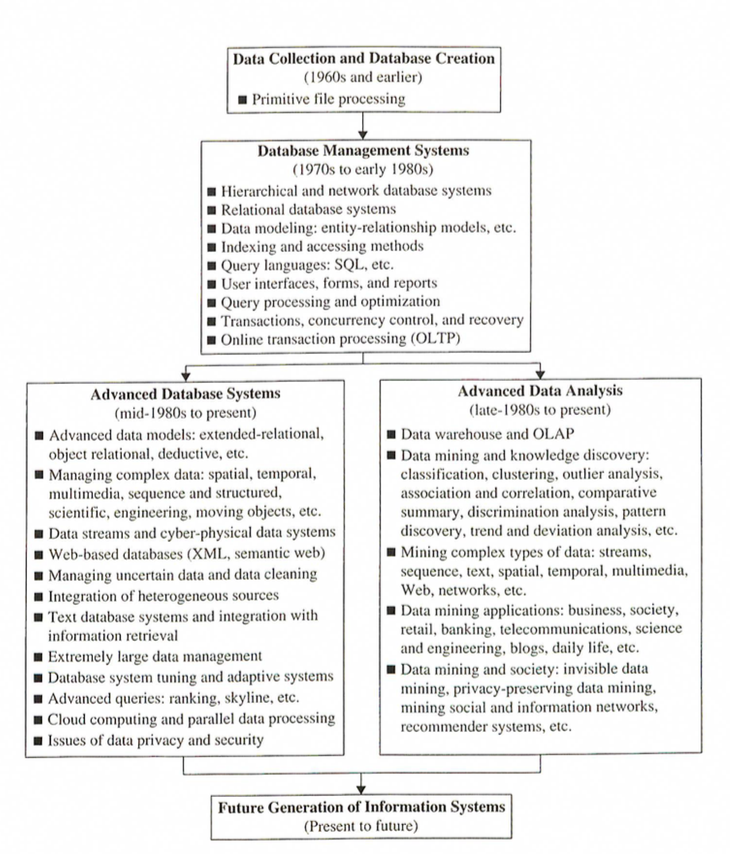
\includegraphics[width=0.6\textwidth]{images/dbevolution}
	\caption{Entwicklung von Datenbank Technologien \cite{DataMiningConceptsAndTechniques}}
	\label{fig:dbevolution}
\end{figure}
%!TEX root=../document.tex

\section{Entwurf und Implementierung von Datenbank Applikationen}
\label{sec:dbapps}

Lorem ipsum dolor sit amet, consectetur adipisicing elit, sed do eiusmod
tempor incididunt ut labore et dolore magna aliqua. Ut enim ad minim veniam,
quis nostrud exercitation ullamco laboris nisi ut aliquip ex ea commodo
consequat. Duis aute irure dolor in reprehenderit in voluptate velit esse
cillum dolore eu fugiat nulla pariatur. Excepteur sint occaecat cupidatat non
proident, sunt in culpa qui officia deserunt mollit anim id est laborum.
%!TEX root=../document.tex

\section{Präsentation von Inhalten mittels Web-Applikation}
\label{sec:webapps}

Lorem ipsum dolor sit amet, consectetur adipisicing elit, sed do eiusmod
tempor incididunt ut labore et dolore magna aliqua. Ut enim ad minim veniam,
quis nostrud exercitation ullamco laboris nisi ut aliquip ex ea commodo
consequat. Duis aute irure dolor in reprehenderit in voluptate velit esse
cillum dolore eu fugiat nulla pariatur. Excepteur sint occaecat cupidatat non
proident, sunt in culpa qui officia deserunt mollit anim id est laborum.
%!TEX root=../document.tex

\section{Datenbankanbindung und Konsistenzerhaltung bei CMS}
\label{sec:cms}

Lorem ipsum dolor sit amet, consectetur adipisicing elit, sed do eiusmod
tempor incididunt ut labore et dolore magna aliqua. Ut enim ad minim veniam,
quis nostrud exercitation ullamco laboris nisi ut aliquip ex ea commodo
consequat. Duis aute irure dolor in reprehenderit in voluptate velit esse
cillum dolore eu fugiat nulla pariatur. Excepteur sint occaecat cupidatat non
proident, sunt in culpa qui officia deserunt mollit anim id est laborum.
%!TEX root=../document.tex

\section{Verwaltung und Optimierung von Informationssystemen}
\label{sec:informationssysteme}

Lorem ipsum dolor sit amet, consectetur adipisicing elit, sed do eiusmod
tempor incididunt ut labore et dolore magna aliqua. Ut enim ad minim veniam,
quis nostrud exercitation ullamco laboris nisi ut aliquip ex ea commodo
consequat. Duis aute irure dolor in reprehenderit in voluptate velit esse
cillum dolore eu fugiat nulla pariatur. Excepteur sint occaecat cupidatat non
proident, sunt in culpa qui officia deserunt mollit anim id est laborum.

%!TEX root=../document.tex

\section{Modellierung und Datenintegration bei mobilen Endgeräten}
\label{sec:mobile}

Lorem ipsum dolor sit amet, consectetur adipisicing elit, sed do eiusmod
tempor incididunt ut labore et dolore magna aliqua. Ut enim ad minim veniam,
quis nostrud exercitation ullamco laboris nisi ut aliquip ex ea commodo
consequat. Duis aute irure dolor in reprehenderit in voluptate velit esse
cillum dolore eu fugiat nulla pariatur. Excepteur sint occaecat cupidatat non
proident, sunt in culpa qui officia deserunt mollit anim id est laborum.
%!TEX root=../document.tex

\section{Datenhaltung und -weitergabe im zwischenbetrieblichen Umfeld}
\label{sec:zwischenbetrieblich}

Lorem ipsum dolor sit amet, consectetur adipisicing elit, sed do eiusmod
tempor incididunt ut labore et dolore magna aliqua. Ut enim ad minim veniam,
quis nostrud exercitation ullamco laboris nisi ut aliquip ex ea commodo
consequat. Duis aute irure dolor in reprehenderit in voluptate velit esse
cillum dolore eu fugiat nulla pariatur. Excepteur sint occaecat cupidatat non
proident, sunt in culpa qui officia deserunt mollit anim id est laborum.

% Reset Autor
\lfoot{}

% BIBL

% For debugging
\nocite{*}
\clearpage
\begingroup
\bibliographystyle{abbrv}
\bibliography{references}
\endgroup

% APPENDENCIES
\clearpage
\pagenumbering{Roman}
\section{Appendix}

\subsection{Figuren}
	\begingroup
		\makeatletter
		\@starttoc{lof}% Print List of Figures
		\makeatother
	\endgroup

\subsection{Tabellen}
	\begingroup
		\makeatletter
		\@starttoc{lot}% Print List of Tables
		\makeatother
	\endgroup

\subsection{Listings}
	\begingroup
		\makeatletter
		\@starttoc{lol}% Print List of Listings lol
		\makeatother
	\endgroup
\end{document}

